\newpage

\section{Loop Invariant Computation and Code Motion}


Loop-Invarian Code Motion (LICM) recognizes computations within a loop that produce the same result each time the loop is executed. 
These computations are called loop-invariant code and can be moved outside the loop body without changing the program semantics. 
The positive effects of LICM are:
\begin{itemize}
\item The shifted loop invariants exhibit a reduced execution frequency.
\item The transformation may shorten variable live ranges leading to a decreased register pressure. This circumstance may in turn reduce the number of required spill code instructions.
\item Moving code outside a loop reduces the loop's size which may be beneficial for the I-cache behavior since more loop code can reside in the cache.
\end{itemize}

Besides these positive effects on the code, LICM may also degrade performance. This is mainly due to two reasons. First, the newly created variables to store the loop-invariant results outside the loop, may increase the register pressure in the loops since their live ranges span across the entire loop nest. As a result, possibly additional spill code is generated. 
Second, LICM might lengthen other paths of the control flow graph. This situation can be observed if the invariants are moved from a less executed to a more frequently executed path, e.g., moving instructions above a loop's zero-trip test.


\subsection{Finding natrual loops}

Not every cicle is a loop in CFG. From a intuitive perspective, a loop must has a single entry and edges must from at least one circle.   

\begin{definition}{Back Edge}
    A back edge is an arc t$\rightarrow$h whose
head h dominates its tail t
\end{definition}

\begin{definition}{Natural Loop}
    The natural loop of a back edge t$\rightarrow$h
    is the smallest set of nodes that
    includes t and h, and has
    no predecessors outside the set,
    except for the predecessors of the header h.
\end{definition}

\begin{definition}{Reducible}
A flow graph is reducible if every retreating edge in any DFST (Deep-First Spanning Tree) for that flow graph is a back edge.
\end{definition}



\paragraph{Testing reducibility} Take any DFST for the flow graph, remove the back edges, and check that the result is acyclic.

\begin{figure}[H]
    \centering
    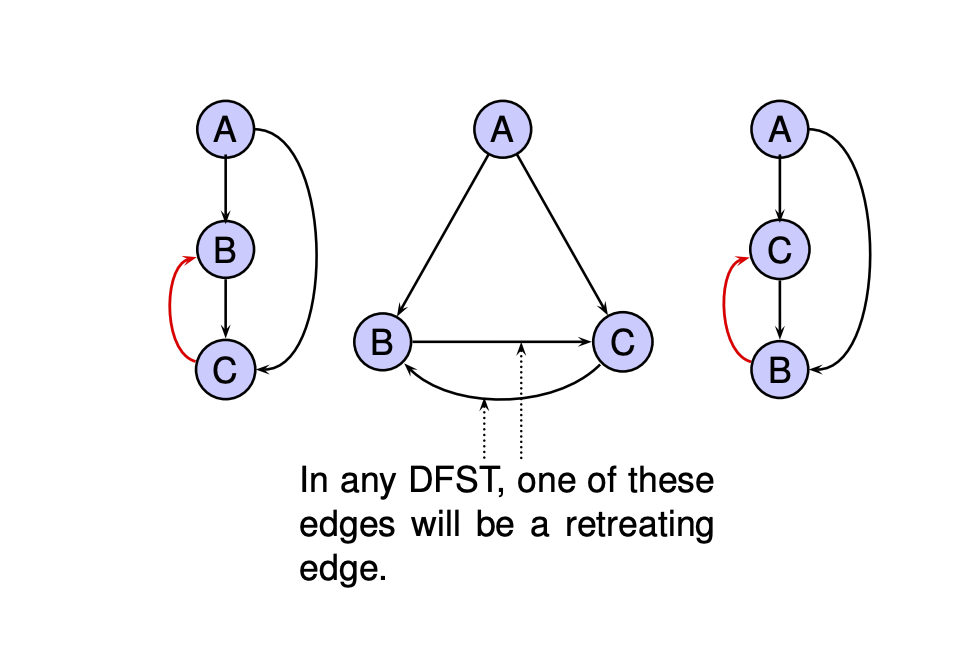
\includegraphics[width=0.5\textwidth]{DFST.png}
    \caption{Example: Nonreducible Graph }
    \label{fig:DFST}
\end{figure}

\subsection{Algorithm to Find Natural Loops}

\subsubsection{Step 1. Finding Dominators}

We can formulate this as Data Flow Analysis problem. Since Node d dominates node n in a graph (d dom n)
if every path from the start node to n goes through d. So if d dom n iff iff d dom p for all pred p of n.
\begin{center}
 \begin{tabular}{|c|c|}
\hline Direction & Forward\\
\hline Values & Basic Blocks\\
\hline Meet operator & \( \cap \)\\
\hline Top(T) & Universal Set\\
\hline Bottom & $\phi$\\
\hline Boundary condition for entry node & $\phi$ \\  
\hline Initialization for internal nodes & \(\mathrm{T}\) \\
\hline Finited escending chain? &\checkmark  \\
\hline Transferfunction  & $\text { OUT }[\mathbf{b}]=\{\mathbf{b}\} \cup\left(\cap_{\{\boldsymbol{p}=\boldsymbol{p r e d}(\boldsymbol{b})\}} \text { OUT }[\mathbf{p}]\right)$ \\
\hline Monotone\&Distributive?  & \checkmark \\
\hline
\end{tabular}  
\end{center}


With rPostorder, most flow graphs (reducible flow graphs) converge in 1 pass. 


\begin{figure}[H]
    \centering
    \begin{subfigure}{0.3\textwidth}
    \centering
        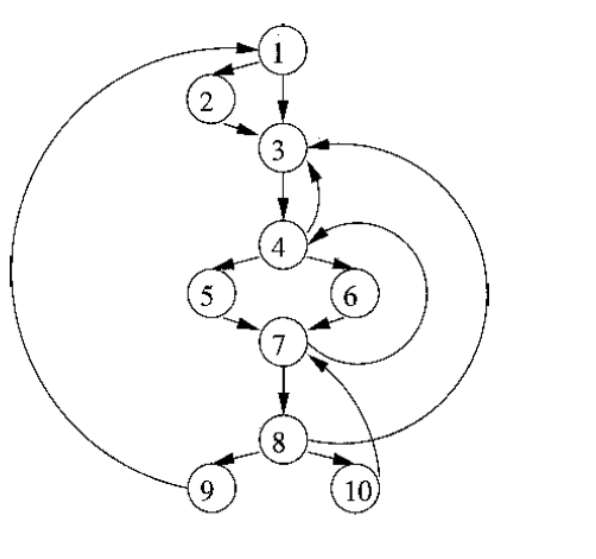
\includegraphics[width=\textwidth]{p61.png}
        \caption{CFG.}
        \label{fig:p61}
    \end{subfigure}
    \begin{subfigure}{0.3\textwidth}
    \centering
        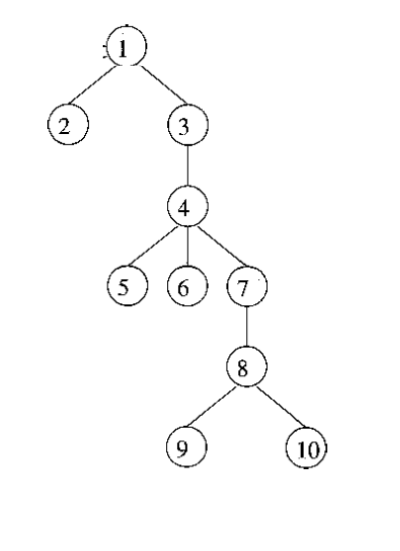
\includegraphics[width=\textwidth]{p62.png}
        \caption{Dominance Tree of the corresponding CFG.}
        \label{fig:p62}
    \end{subfigure}
    
    \caption{An example of Dominance tree.}
       \label{fig:p51-58}
\end{figure}



\subsubsection{Step 2. Finding Back Edges}

\paragraph{Depth-first spanning tree}
Edges traversed in a depth-first search of the flow graph form a depth-first spanning tree. We categorize edges in CFG as follows:
\begin{itemize}
    \item Forward edges (node to proper descendant).
    \item Retreating edges (node to ancestor).
    \item Cross edges (between two nodes, neither of which is an ancestor of the other.)
\end{itemize}

This is something difficult to understand. Let's make it simpler. We can number each node when we visit it. So each edge should be satisfied the following property:


\begin{center}
\begin{tabular}{|c|c|}
\hline Forward/Advancing edges  \( n_1 \rightarrow n_2\) & num($n_1$) $<$ num($n_2$) and  $n_1$ is ancestor of  $n_2$\\
\hline Cross edges  \( n_1 \rightarrow n_2\)& num($n_1$) $>$ num($n_2$) and neither  $n_1$ is ancestor of  $n_2$ nor $n_2$ is ancestor of  $n_1$ \\
\hline Retreating edges  \( n_1 \rightarrow n_2\) & num($n_1$) $>$ num($n_2$) and  $n_2$ is ancestor of  $n_1$\\
\hline
\end{tabular}  
\end{center}





Of these edges, only retreating edges go from high to low in DF order.



\paragraph{Algorithm}

\begin{itemize}
    \item Perform a depth first search
    \item For each retreating edge \(t \rightarrow h\), check if h is in t$^\prime$s dominator list. If so,  \(t \rightarrow h\) is a back edge.
\end{itemize}


\begin{figure}[H]
    \centering
    \begin{subfigure}{0.3\textwidth}
    \centering
        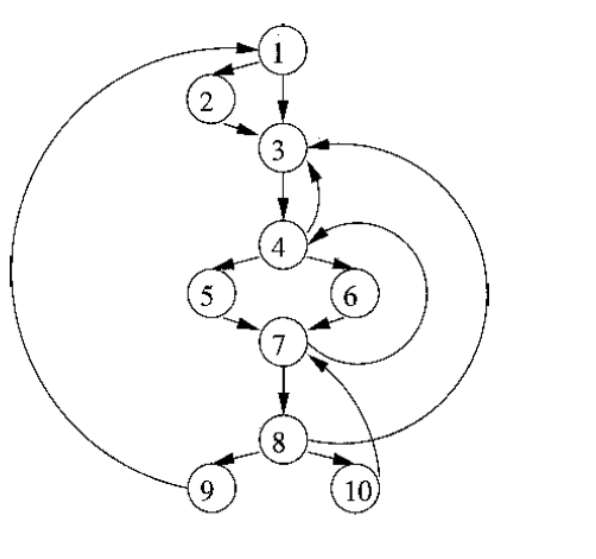
\includegraphics[width=\textwidth]{p61.png}
        \caption{CFG.}
        \label{fig:p61}
    \end{subfigure}
    \begin{subfigure}{0.3\textwidth}
    \centering
        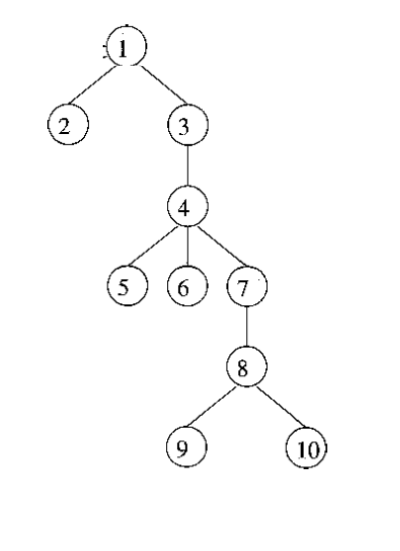
\includegraphics[width=\textwidth]{p62.png}
        \caption{Dominance Tree of the corresponding CFG.}
        \label{fig:p62}
    \end{subfigure}
    \begin{subfigure}{0.3\textwidth}
        \centering
            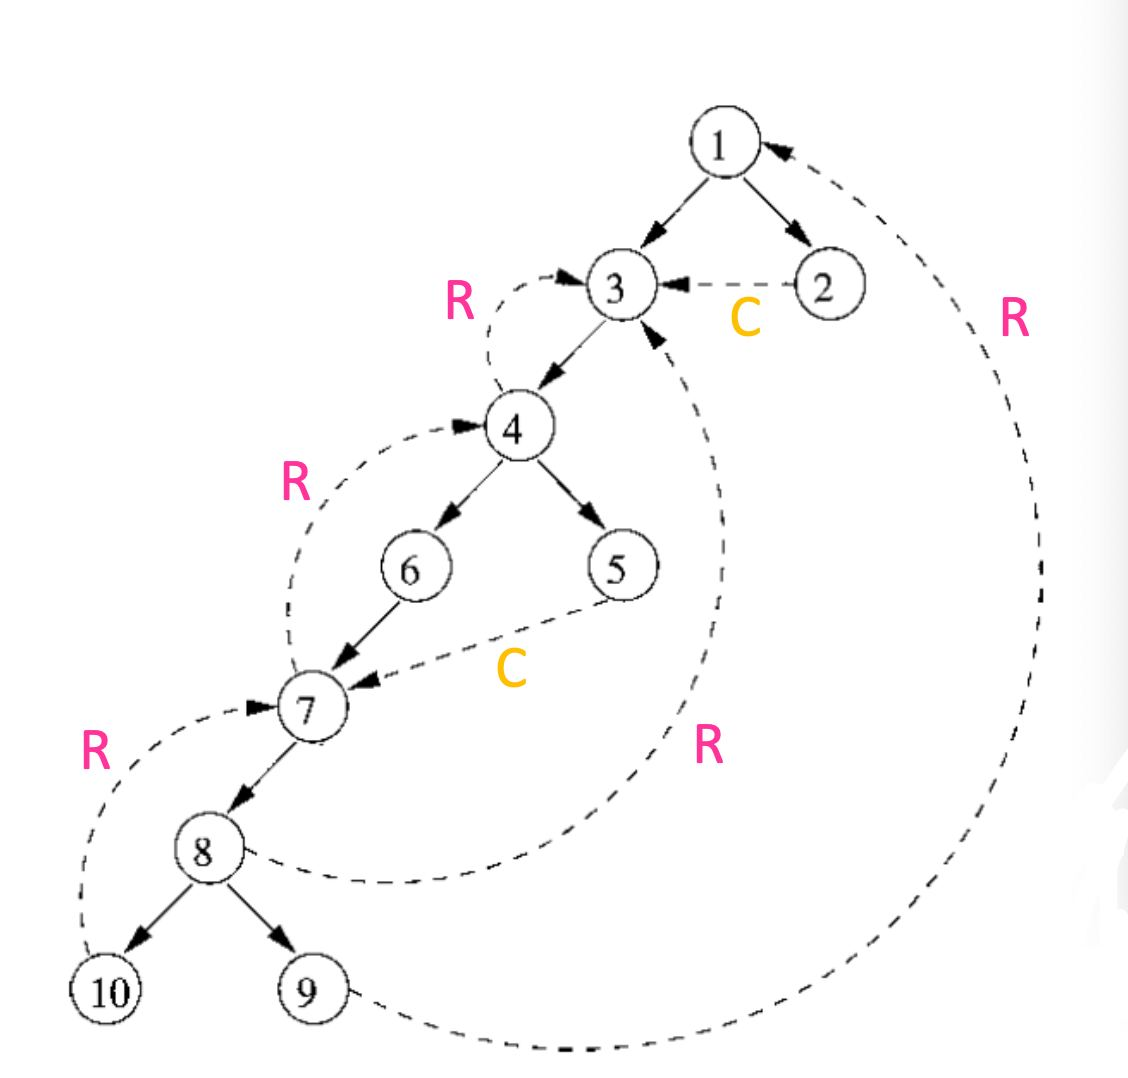
\includegraphics[width=\textwidth]{p63.jpg}
            \caption{{\color{red} R} means back edges and {\color{orange} C} means cross edge.}
            \label{fig:p62}
        \end{subfigure}
    \caption{An example of Back Eges.}
       \label{fig:p51-58}
\end{figure}

\subsubsection{Step 3. Constructing Natural Loops}

\paragraph{Algorithm} For each back edge $t\rightarrow h$:

\begin{itemize}
    \item delete h from the flow graph
    \item find those nodes that can reach t
(those nodes plus h form the natural loop of \(t \rightarrow h\))
\end{itemize}

\begin{figure}[H]
    \centering
     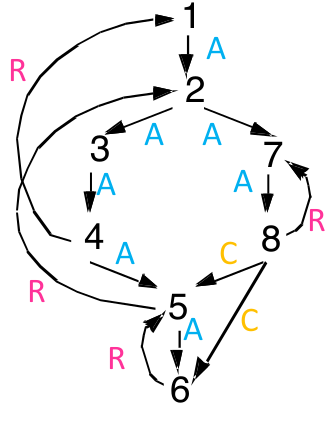
\includegraphics[width=0.3\textwidth]{p64.png}
         \caption{For this flow graph, for back edge 8 $\rightarrow$ 7, natrual loop is \{ 7,8 \}, for back edge 5 $\rightarrow$ 2, natrual loop is \{ 2,3,4,5,6,7,8 \},back edge 4 $\rightarrow$ 1, natrual loop is \{ 1,2,3,4,5,6,7,8\}.}
         \label{fig:p64}
\end{figure}

\subsection{Inner Loops}

If two different loops don't have ths same header, they are either disjoint or one is entirely contained the other (inner loop is the one that contains no other loop.).
If two loops share the same header shown in Figure \ref{fig:p65}, it is hard to tell which is the inner loop. But we can combine and treat as one loop.


\begin{figure}[H]
    \centering
     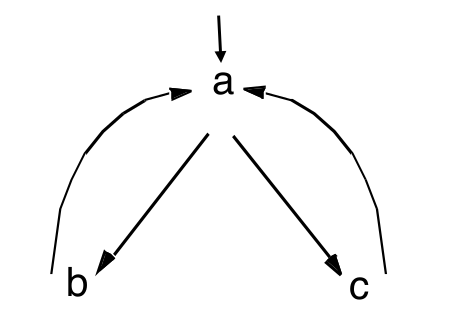
\includegraphics[width=0.3\textwidth]{p65.png}
         \caption{Two loops share the same header.}
         \label{fig:p65}
\end{figure}






\subsection{Loop-Invariant Computation and Code Motion}

\begin{definition}{Loop-Invariant Computation}
    A loop-invariant computation is a computation whose value doesn't change as long as control stays within the loop. 
    loop invariant whose operands are defined outside loop or invariant themselves.
\end{definition}


\begin{figure}[H]
    \centering
     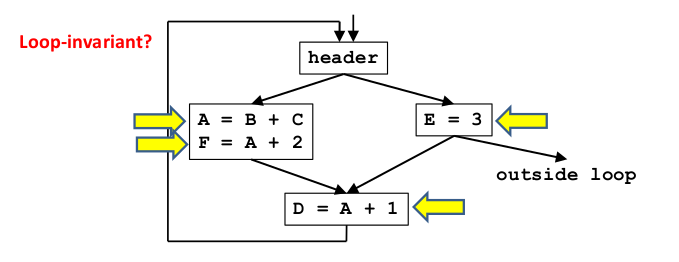
\includegraphics[width=0.7\textwidth]{p66.png}
         \caption{For this CFG, \texttt{A = B+C, F=A+2, E=3} are Loop-Invariant Computation, but \texttt{D = A + 1} is not. }
         \label{fig:p66}
\end{figure}



Not all loop invariant instructions can be moved to preheader.


\subsection{LICM Algorithm}

\begin{itemize}
\item Find invariant expressions
\item Conditions for code motion
\item Code transformation
\end{itemize}



\subsection{Find invariant expressions}


\begin{itemize}
    \item Compute reaching definitions
    \item Repeat: mark \texttt{A = B + C} as invariant if
    \begin{itemize}
        \item All reaching definitions of B are outside the loop or
        there is exactly one reaching definition for B and it is from a loop-invariant statement inside the loop.  
        \item Check the same for C.
        \end{itemize}
    \item Code transformation
    \end{itemize}


    \begin{figure}[H]
        \centering
         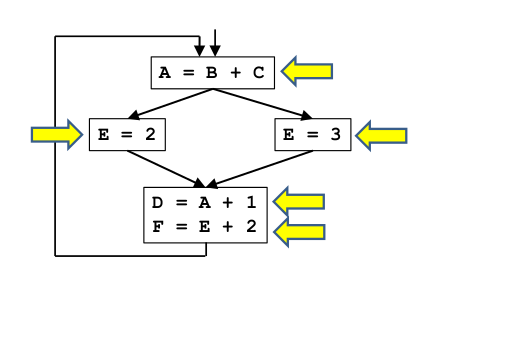
\includegraphics[width=0.7\textwidth]{p67.png}
             \caption{For this CFG, \texttt{A = B+C, E = 2, E = 3, D = A + 1} are Loop-Invariant Computation, but \texttt{F = E + 2} is not because two definitions of E reach \texttt{F = E + 2}. }
             \label{fig:p67}
    \end{figure}


\subsection{Conditions for Code Motion}




\begin{algorithm}[H]
    \caption{Code Motion Algorithm}\label{alg:Code Motion Algorithm}
    \begin{algorithmic}
    \State{Given: a set of nodes in a loop}
    \State{Compute reaching definitions}
    \State{Compute loop invariant computation}
    \State{Compute dominators}
    \State{Find the exits of the loop (i.e. nodes with successor outside loop)}
    \State{Candidate statement for code motion:}
    \State{\,\,\,\,\,\,\,\, loop invariant}
    \State{\,\,\,\,\,\,\,\, in blocks that dominate all the exits of the loop shown in \ref{fig:p68}}
    \State{\,\,\,\,\,\,\,\, assign to variable not assigned to elsewhere in the loop}
    \State{\,\,\,\,\,\,\,\, in blocks that dominate all blocks in the loop that use the variable assigned shown in \ref{fig:p69}}
    \State{Perform a depth-first search of the blocks}
    \State{\,\,\,\,\,\,\,\, Move candidate to preheader if all the invariant operations it depends upon
    have been moved}
    \end{algorithmic}
    \end{algorithm}


\begin{figure}[H]
    \centering
     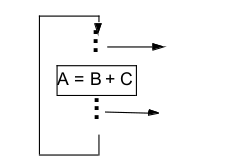
\includegraphics[width=0.4\textwidth]{p68.png}
         \caption{It is not safe to move \texttt{A = B + C} outside the loop because we can jump of the loop before executing \texttt{A = B + C}}
         \label{fig:p68}
\end{figure}

\begin{figure}[H]
    \centering
     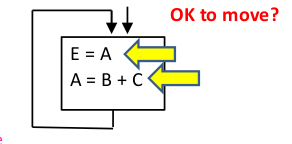
\includegraphics[width=0.4\textwidth]{p69.png}
         \caption{It is not safe to move \texttt{A = B + C} outside the loop because if so, the first time we enter the loop \texttt{E = A} will not the same as before.}
         \label{fig:p69}
\end{figure}

\begin{figure}[H]
    \centering
     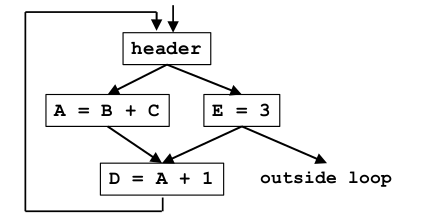
\includegraphics[width=0.4\textwidth]{p70.png}
         \caption{Only \texttt{E = 3} can be moved outside the loop.}
         \label{fig:p70}
\end{figure}


\begin{figure}[H]
    \centering
     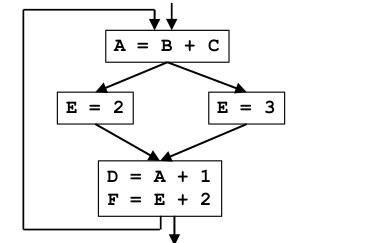
\includegraphics[width=0.4\textwidth]{p71.png}
         \caption{Only \texttt{A = B + C , D = A + 1} can be moved outside the loop.}
         \label{fig:p71}
\end{figure}

\subsection{More Aggressive Optimizations}

\subsubsection{Gamble on: most loops get executed}

We can relax constraint of dominating all exits on some cases.

\begin{figure}[H]
    \centering
     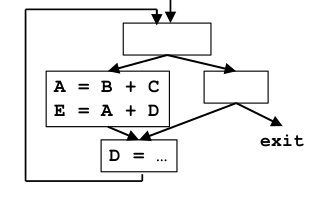
\includegraphics[width=0.4\textwidth]{p72.png}
         \caption{\texttt{A = B + C} cannot be removed outside the loop because it doesn't dominat the exit. But if A is not live after the loop, we can actually move it to the preheader. The only thing we need to consider is that this statement can cause an exception.}
         \label{fig:p72}
\end{figure}


\subsubsection{Landing pads}
\texttt{while} loop is not very convenient for optimization since it checks before entering the loop.  We can use landing pads to solve this.

\begin{figure}[H]
    \centering
     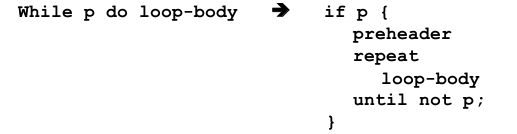
\includegraphics[width=0.6\textwidth]{p73.png}
         \caption{Transforms for while loops.}
         \label{fig:p73}
\end{figure}





\subsection{Summary}

It's common some natrual loops share the same header \ref{fig:p245-6}, from optimization's perspective, we can combine them as a whole. 


\begin{figure}[H]
    \centering
    \begin{subfigure}{0.3\textwidth}
    \centering
        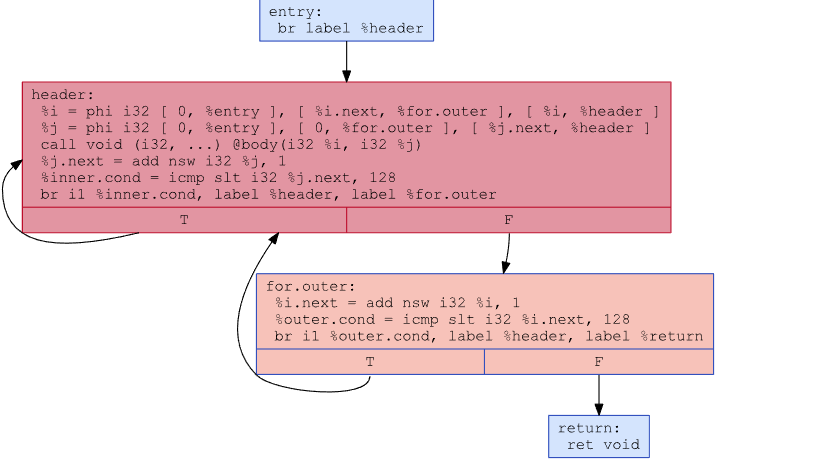
\includegraphics[width=\textwidth]{p245.png}
        \caption{}
        \label{fig:p256}
    \end{subfigure}
    \begin{subfigure}{0.4\textwidth}
    \centering
        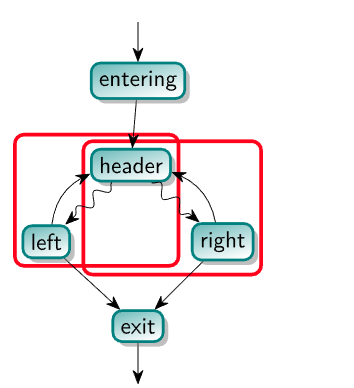
\includegraphics[width=\textwidth]{p246.png}
        \caption{}
        \label{fig:p246}
    \end{subfigure}
    
    \caption{}
       \label{fig:p245-6}
\end{figure}


\begin{lstlisting}[language=C,frame=single, caption=,label = LICM:expression1]
for (int i = 0; i < 128; ++i)
    for (int j = 0; j < 128; ++j)
      body(i,j);
  
\end{lstlisting}



